\documentclass[10pt,twocolumn]{report}
\usepackage{ctex}
\usepackage[utf8]{inputenc}
\usepackage{amsmath}
\usepackage{amssymb}
\usepackage{xcolor}
\usepackage{graphicx}
\usepackage[margin=0.1cm]{geometry} % 设置页边距为 0.5cm，尽可能扩大可用区域
\usepackage{setspace}
\renewcommand{\baselinestretch}{1} % 设置行间距为单倍行距
\usepackage{float}
\usepackage{wrapfig}
\usepackage[utf8]{inputenc}
\usepackage[T1]{fontenc}
\usepackage{ctex}
\usepackage{amsmath}
\usepackage{amssymb}
\usepackage{xcolor}
\usepackage{graphicx}
\usepackage{float}
\usepackage{lmodern}
\usepackage{mathrsfs}
\usepackage{lipsum}
\usepackage{array} 
\usepackage{amsmath}    % 数学公式
\usepackage{booktabs}   % 专业表格
\usepackage{multirow}   % 多行表格
\usepackage{graphicx}   % 插入图片
\usepackage{siunitx}    % 国际单位
\usepackage{enumitem}   % 列表控制
\usepackage{graphicx}
\usepackage{subcaption} % 支持子图
\usepackage{tikz}
\usepackage{braket}
\usepackage{adjustbox}
\usepackage{footmisc}
\usepackage{array}
\usepackage{multirow}
\usepackage[table]{xcolor}
\usepackage{amsmath}
\usepackage{tcolorbox}
\usepackage{caption}
\usepackage{tabularx}
\captionsetup[figure]{labelformat=empty} % 设置图标题的标签格式为空，即不显示“图 X”
\usepackage{graphicx}
\tcbuselibrary{listings,breakable}
\usepackage{xcolor}
\setlength{\parindent}{0pt}
\captionsetup[figure]{skip=0pt}
\usepackage{array}
\begin{document}
	\section{电流图像}
	\subsection{RC}
	\begin{figure}[H]
		\centering
		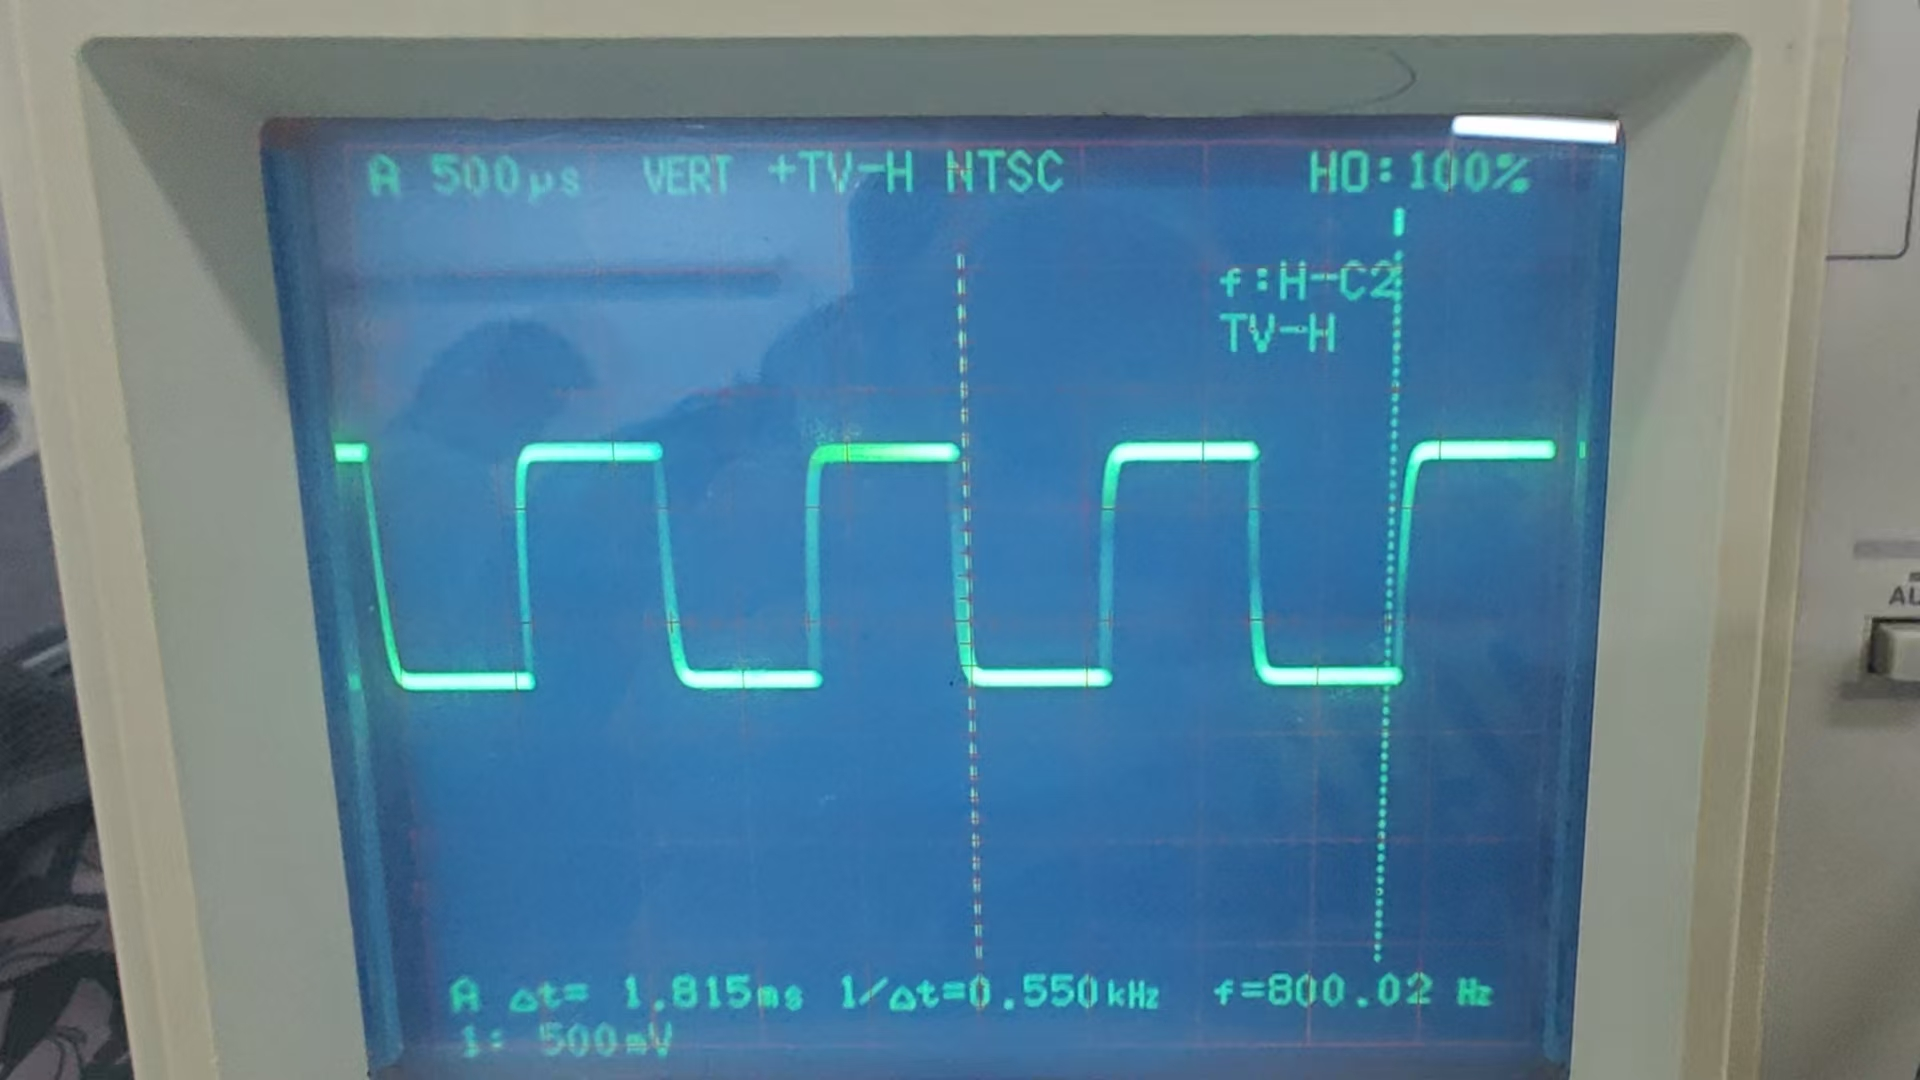
\includegraphics[width=0.55\linewidth]{RC100}
		\caption{$RC100\Omega$}
		\label{fig:rc100}
	\end{figure}
	\begin{figure}[H]
		\centering
		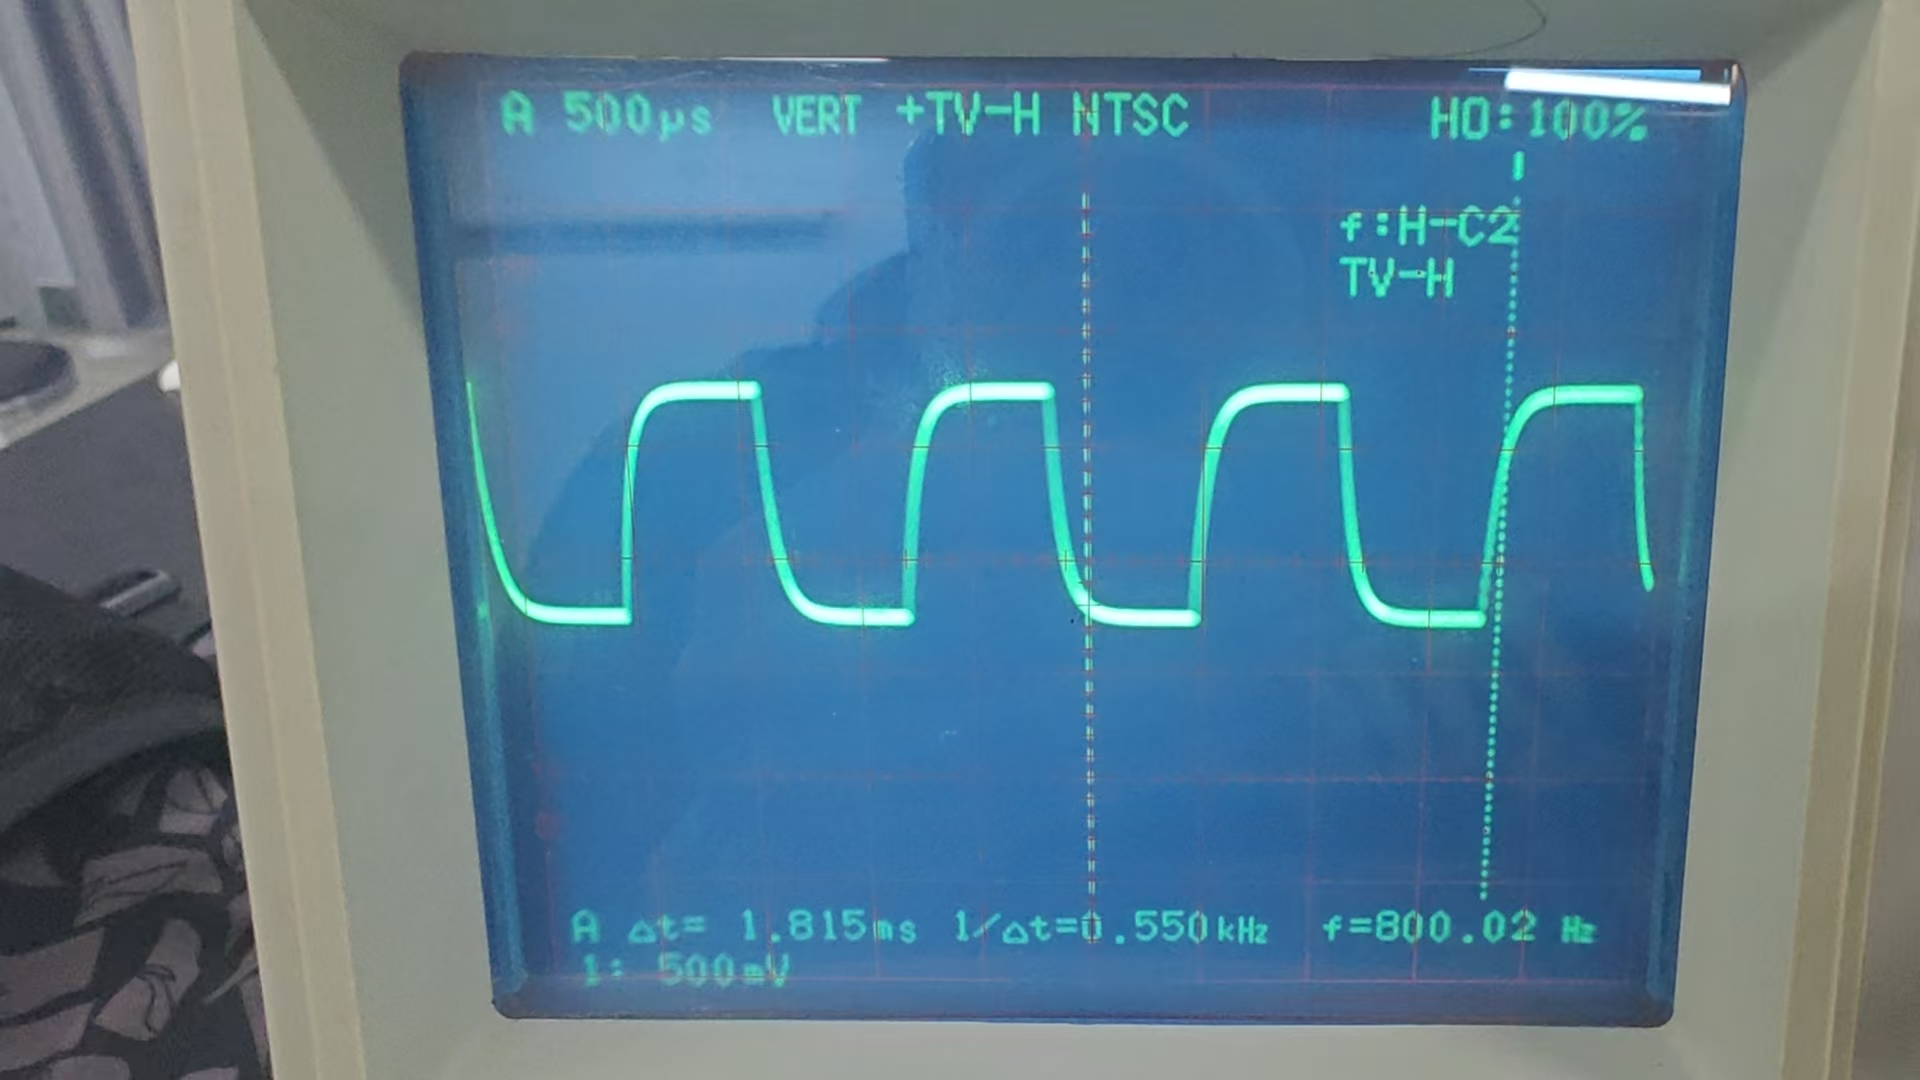
\includegraphics[width=0.55\linewidth]{RC510}
		\caption{$RC510\Omega$}
		\label{fig:rc510}
	\end{figure}
	\begin{figure}[H]
		\centering
		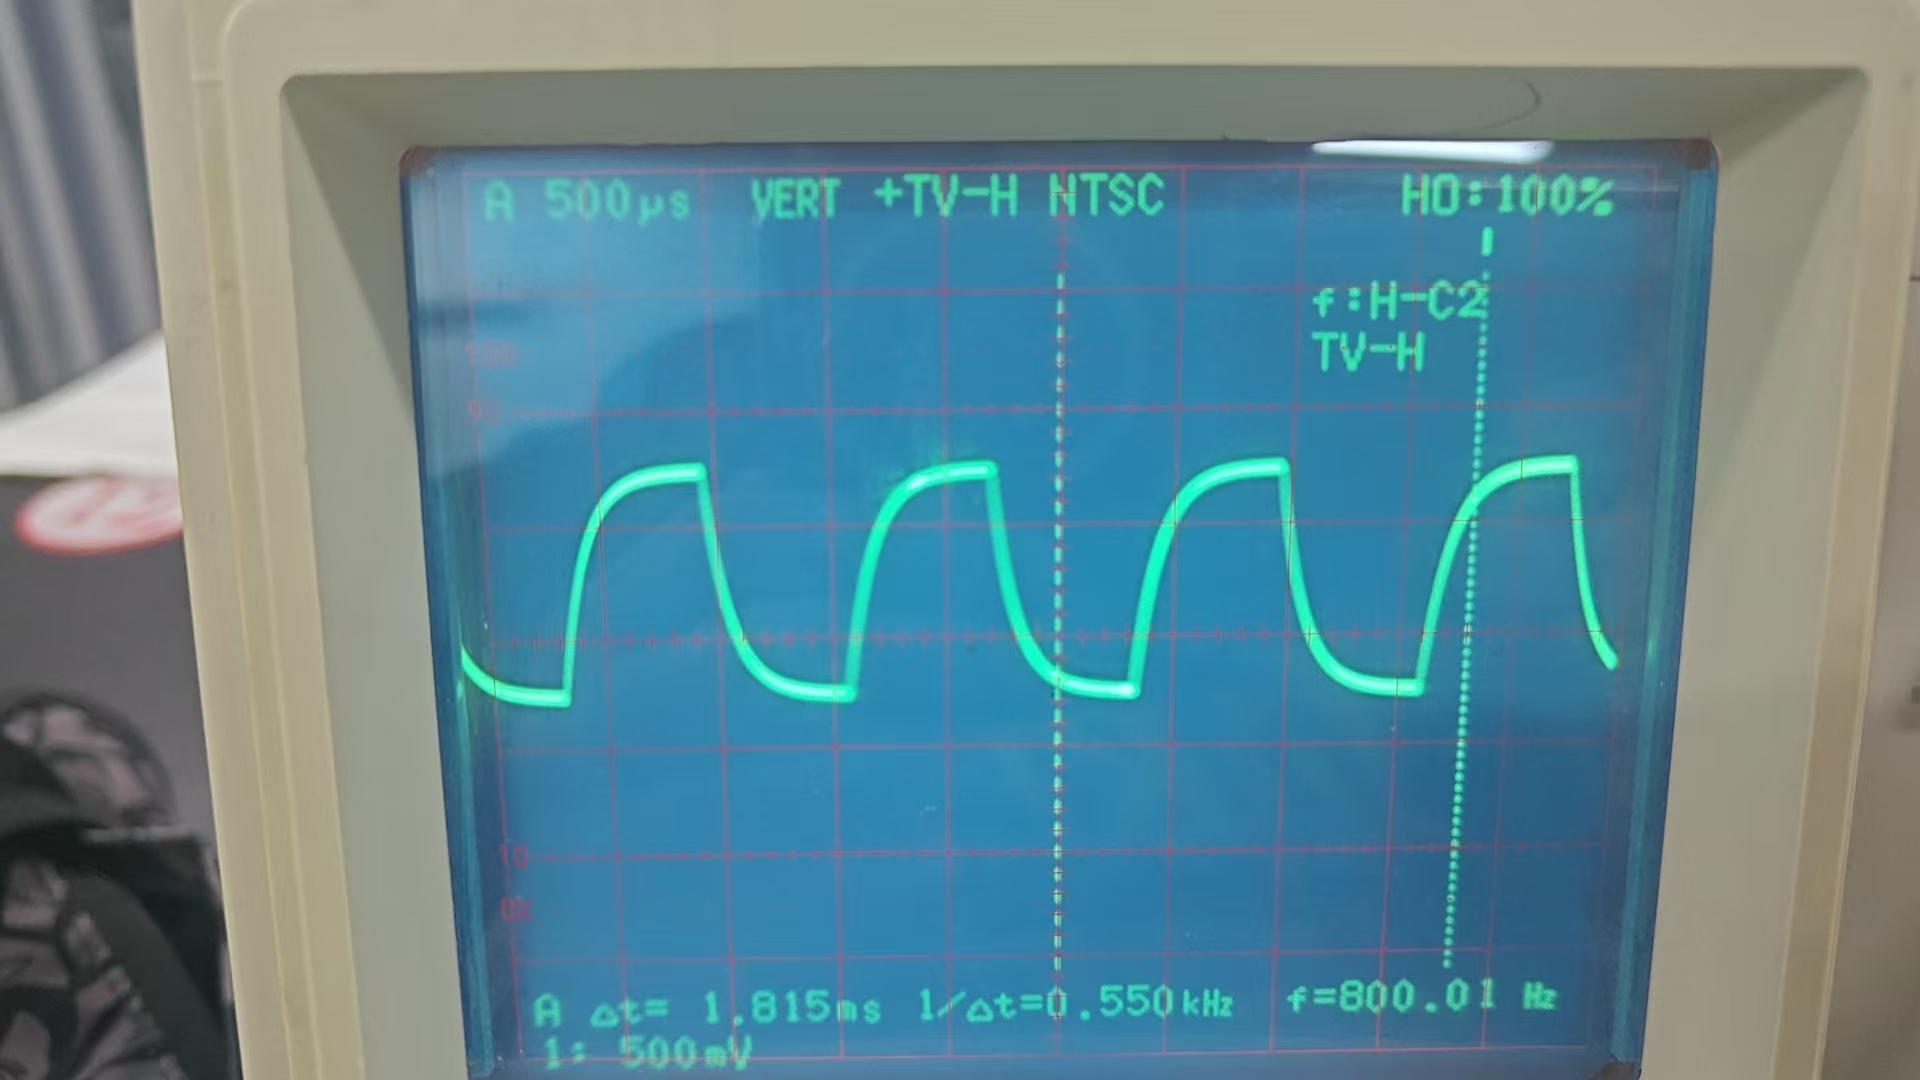
\includegraphics[width=0.55\linewidth]{RC1000}
		\caption{$RC1000\Omega$}
		\label{fig:rc1000}
	\end{figure}
	\begin{figure}[H]
		\centering
		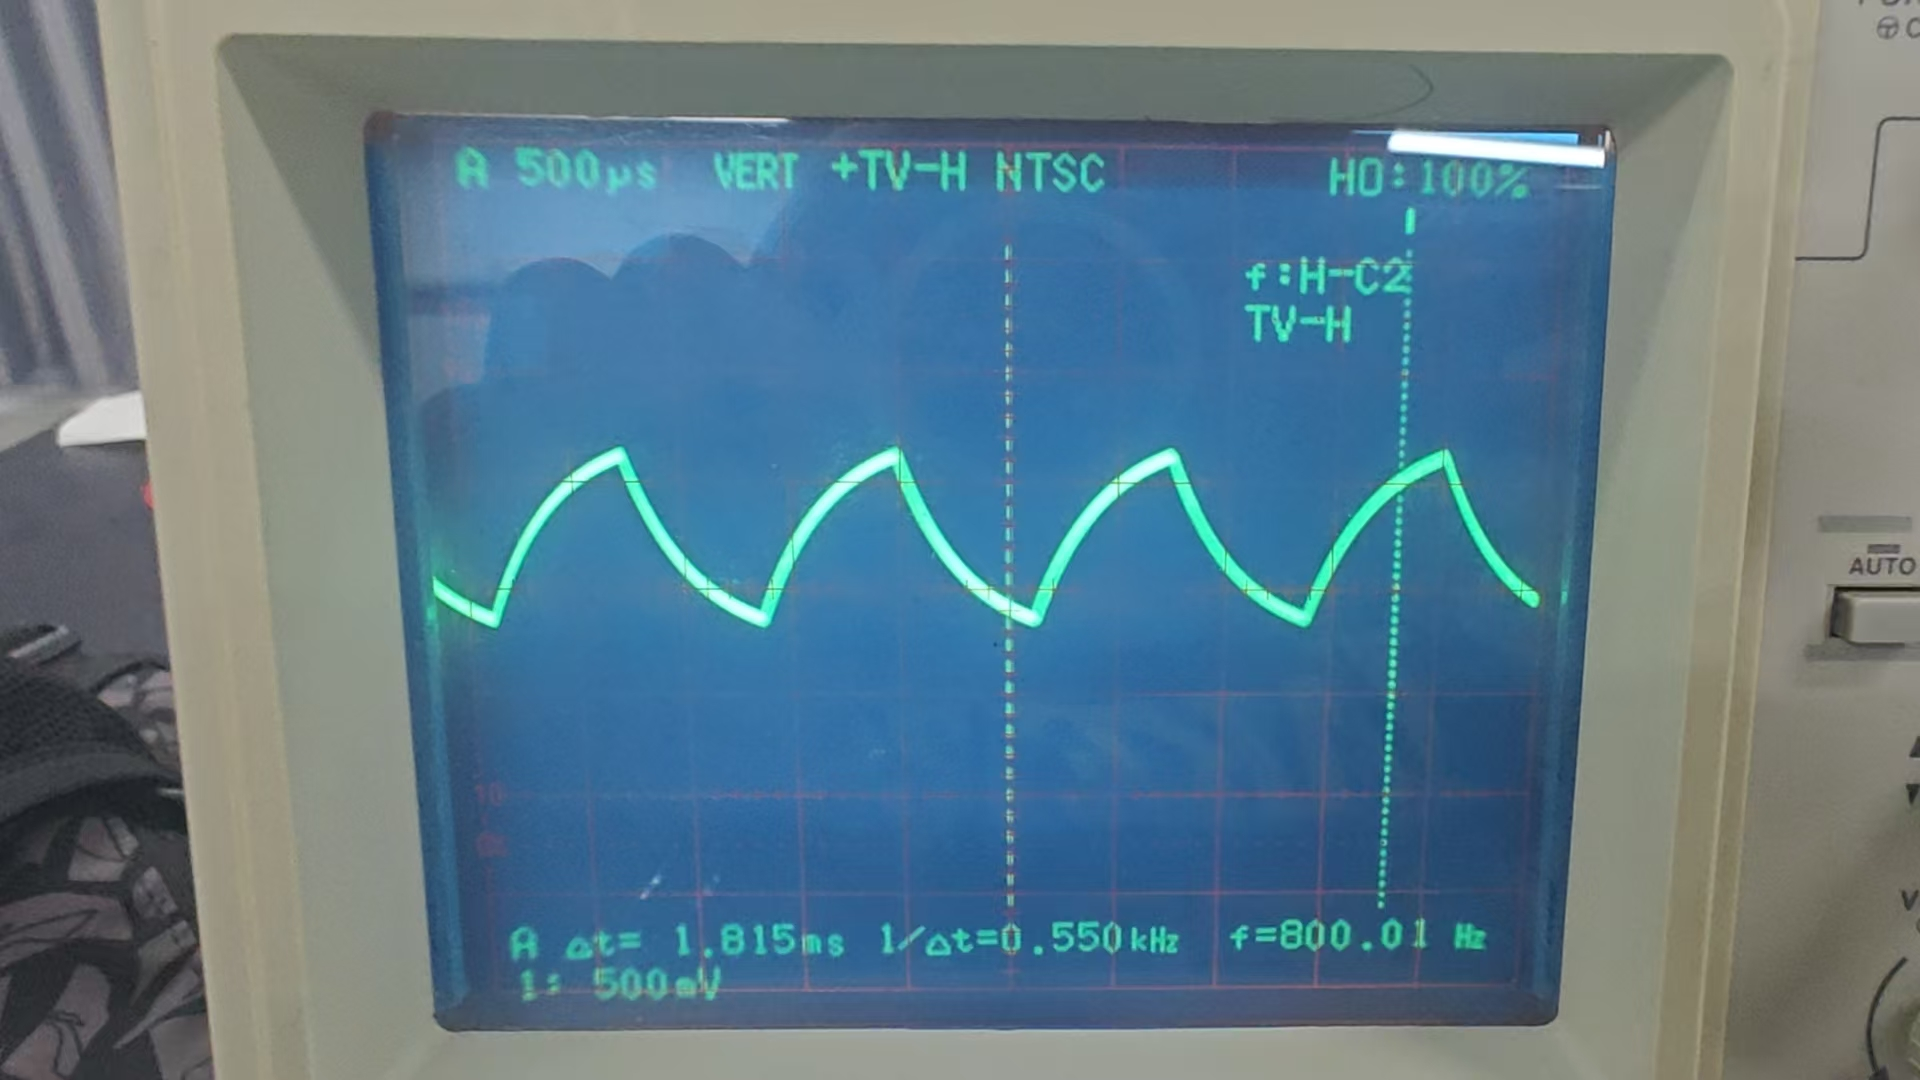
\includegraphics[width=0.55\linewidth]{RC3000}
		\caption{$RC3000\Omega$}
		\label{fig:rc3000}
	\end{figure}
	\subsection{RL}
	\begin{figure}[H]
		\centering
		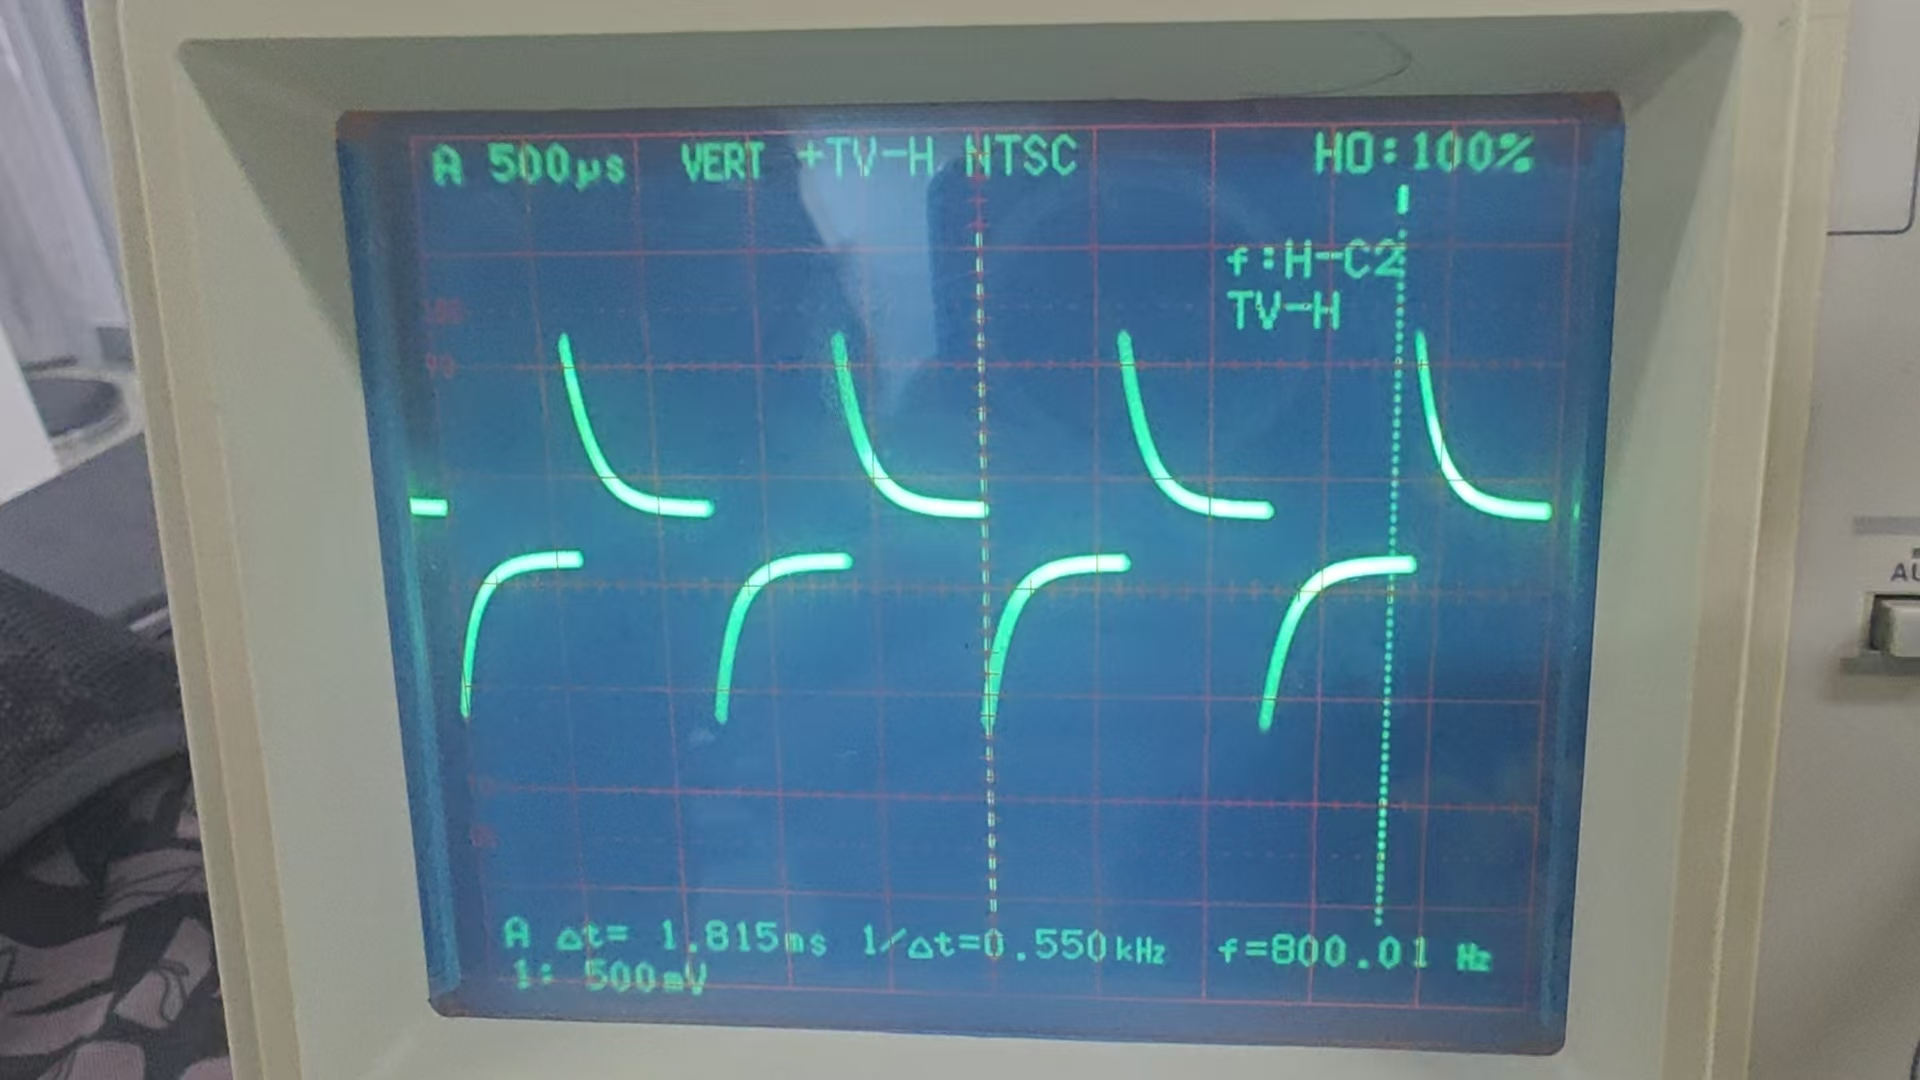
\includegraphics[width=0.55\linewidth]{RL100}
		\caption{$RL100\Omega$}
		\label{fig:rl100}
	\end{figure}
	\begin{figure}[H]
		\centering
		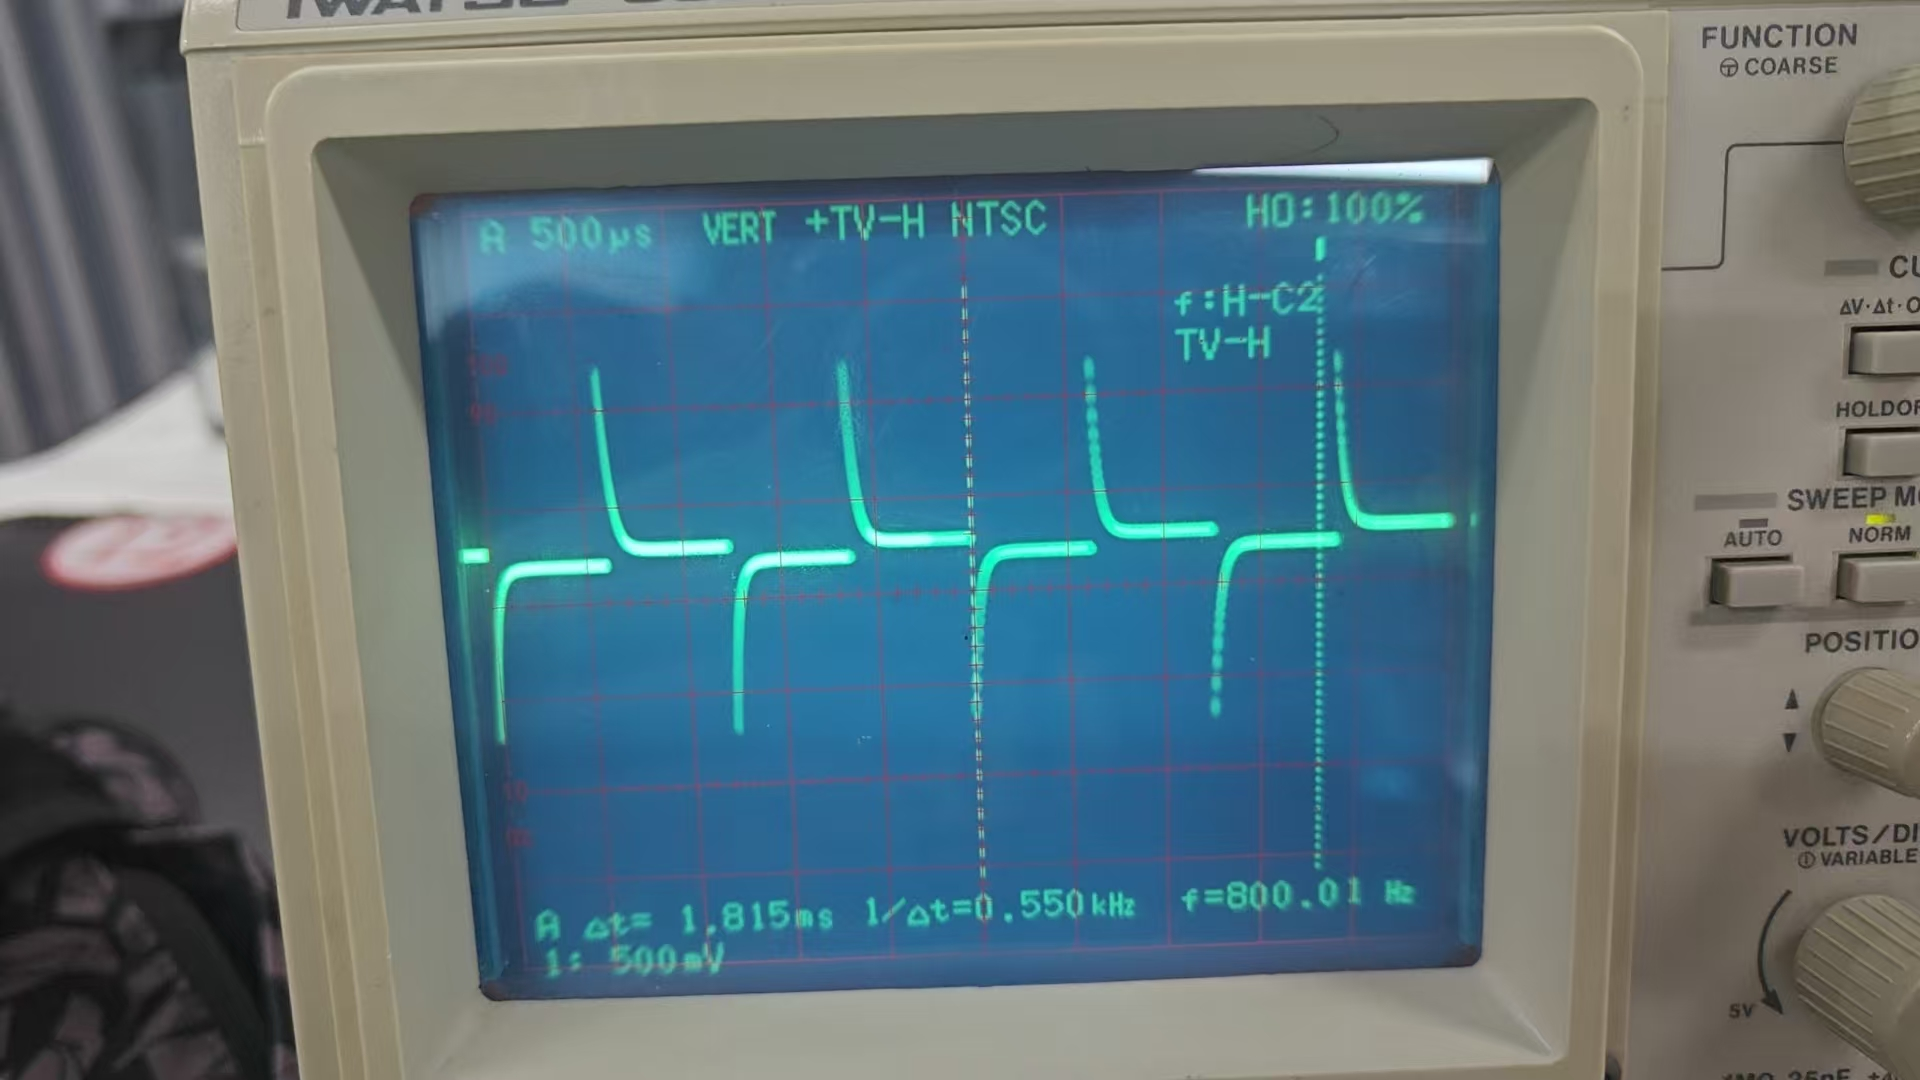
\includegraphics[width=0.55\linewidth]{RL510}
		\caption{$RL510\Omega$}
		\label{fig:rl510}
	\end{figure}
	\begin{figure}[H]
		\centering
		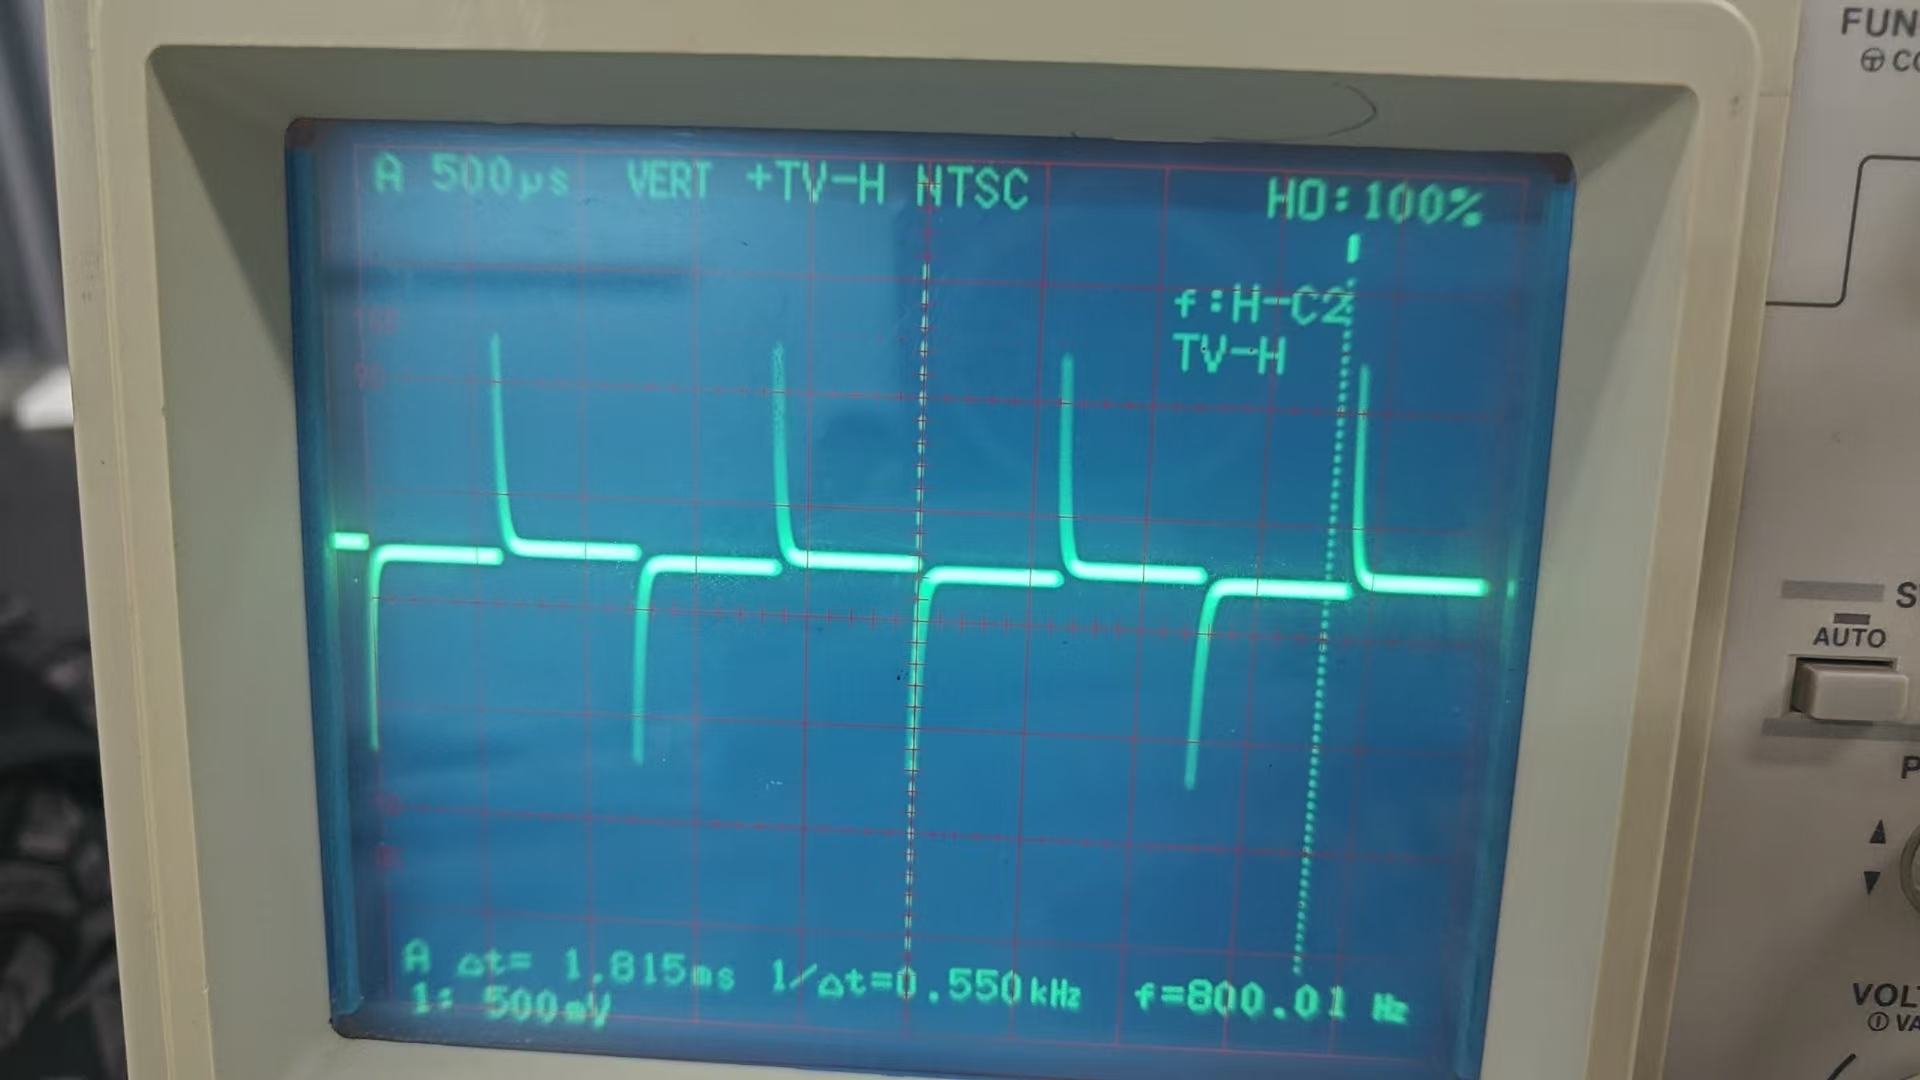
\includegraphics[width=0.55\linewidth]{RL1000}
		\caption{$RL1000\Omega$}
		\label{fig:rl1000}
	\end{figure}
	\begin{figure}[H]
		\centering
		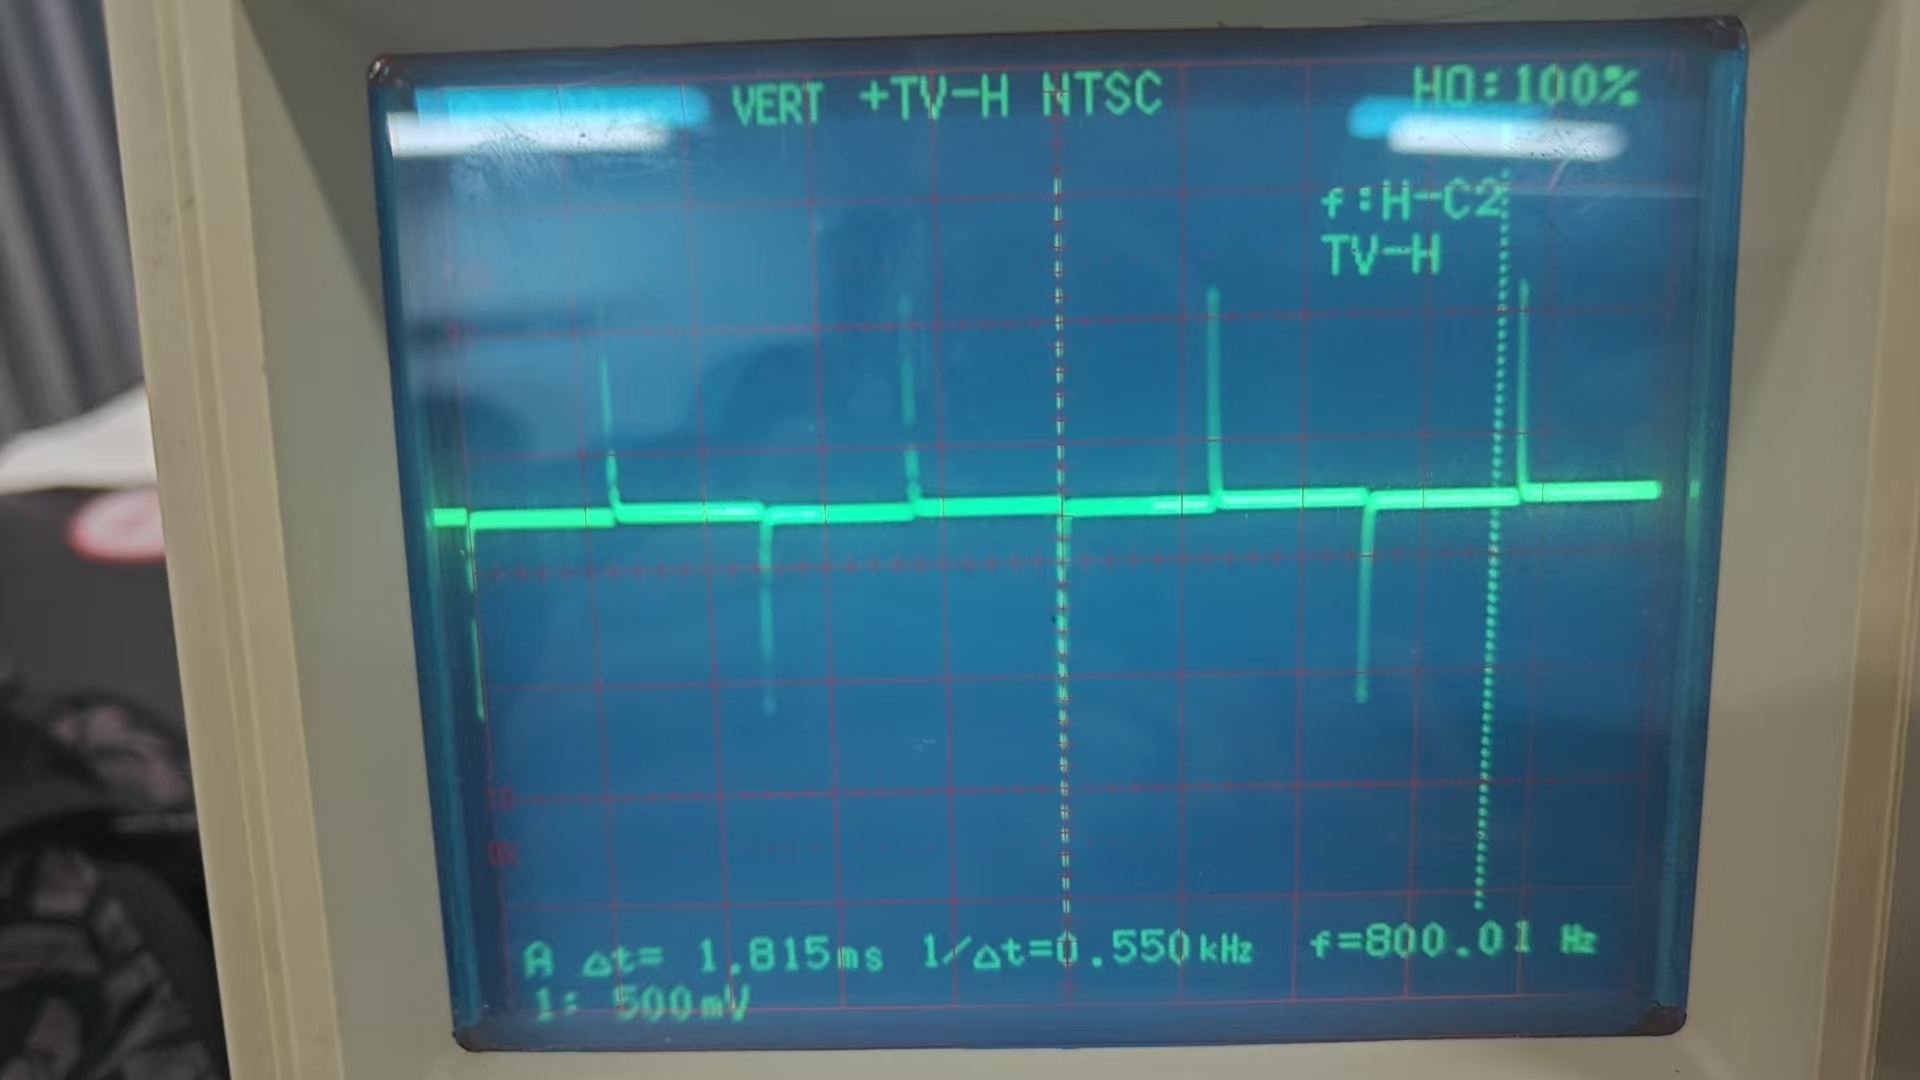
\includegraphics[width=0.55\linewidth]{RL3000}
		\caption{$RL3000\Omega$}
		\label{fig:rl3000}
	\end{figure}
	\subsection{RLC}
	\begin{figure}[H]
		\centering
		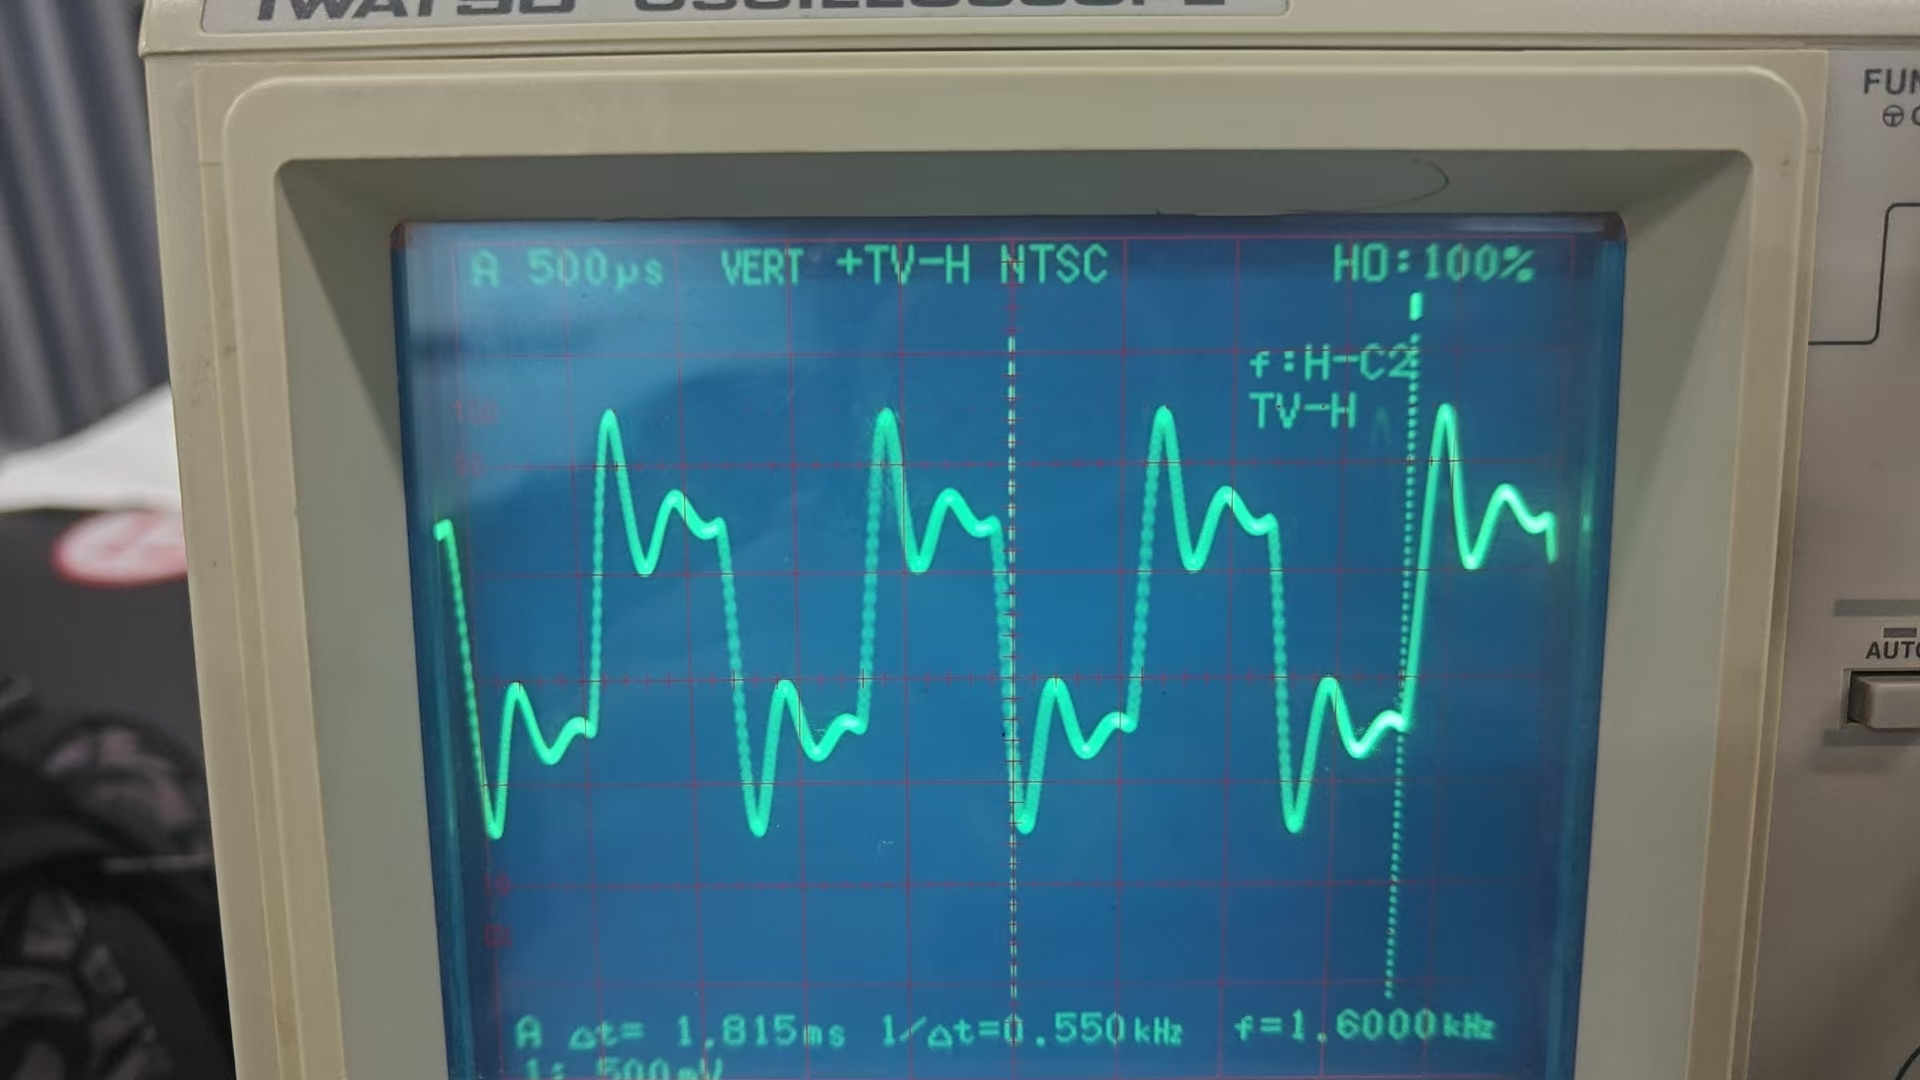
\includegraphics[width=0.55\linewidth]{RLC100}
		\caption{$RLC100\Omega$}
		\label{fig:rlc100}
	\end{figure}
	\begin{figure}[H]
		\centering
		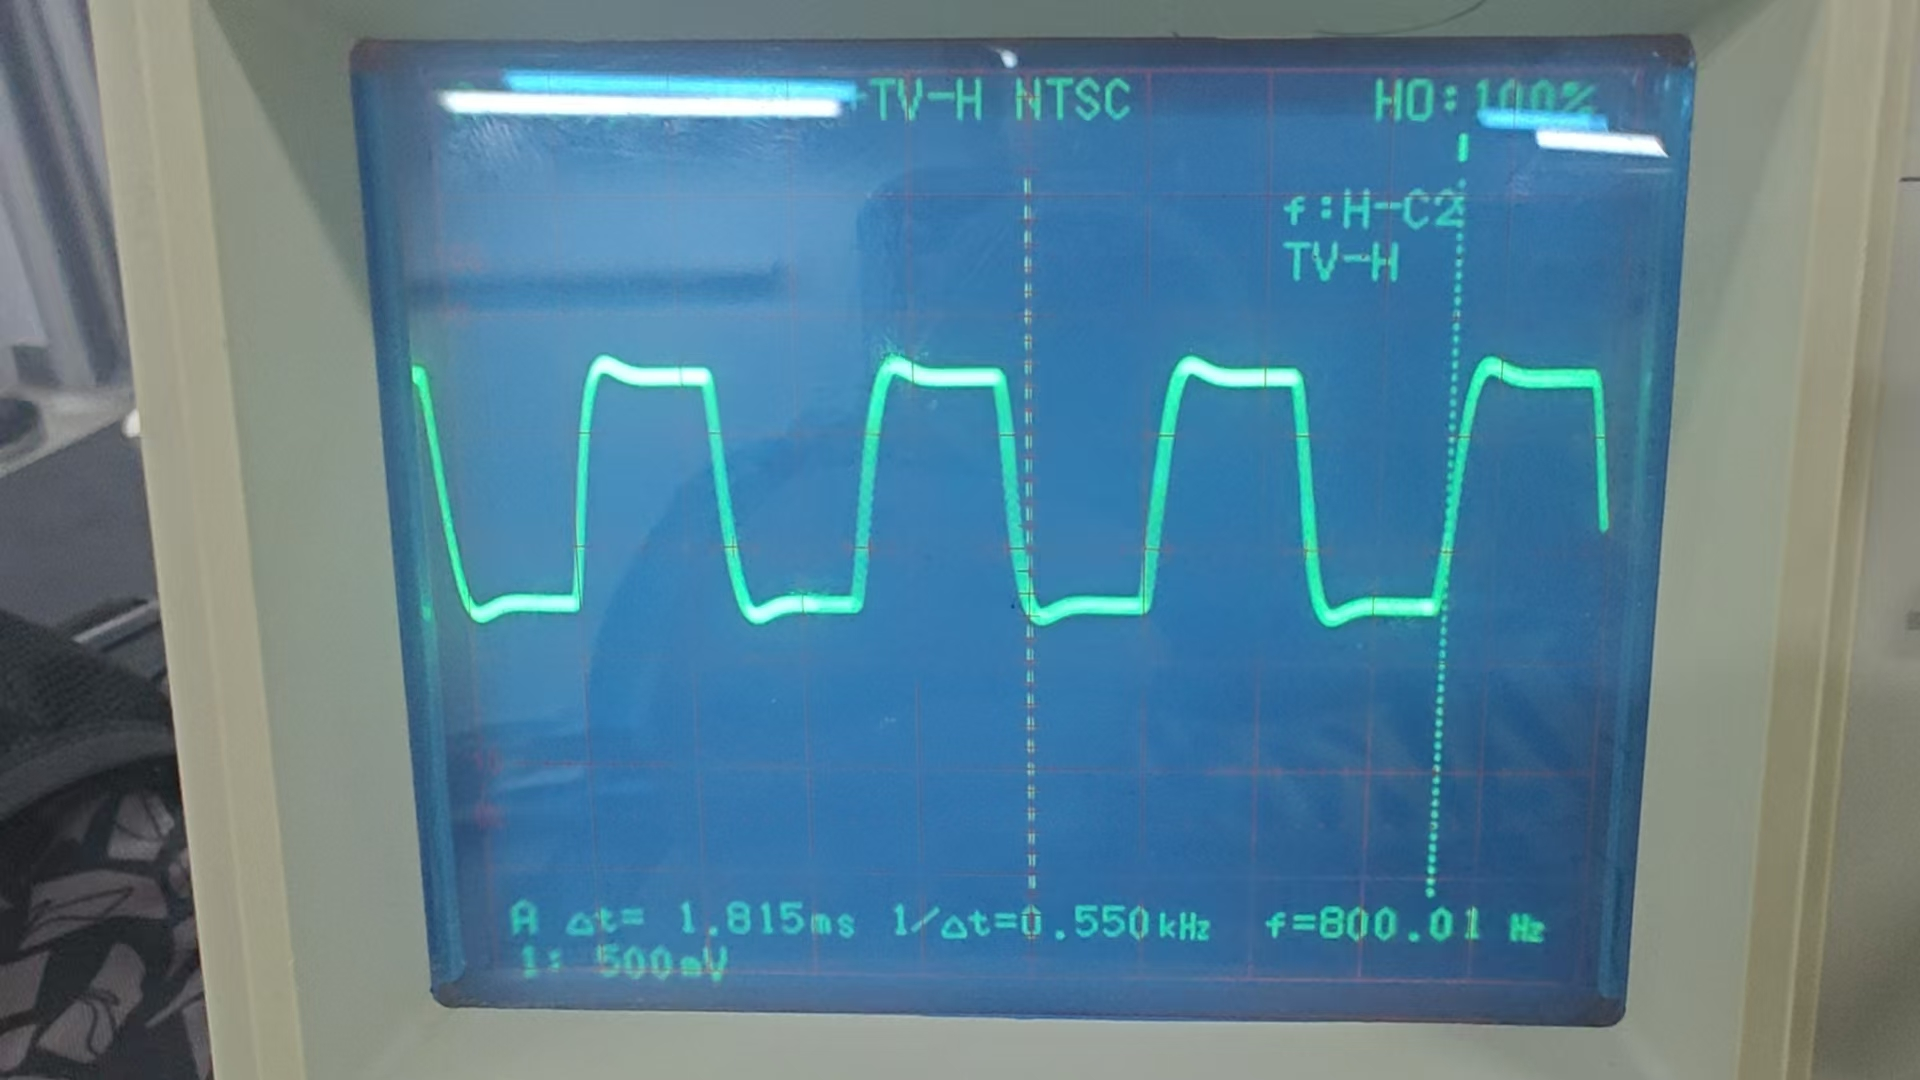
\includegraphics[width=0.55\linewidth]{RLC510}
		\caption{$RLC510\Omega$}
		\label{fig:rlc510}
	\end{figure}
	\begin{figure}[H]
		\centering
		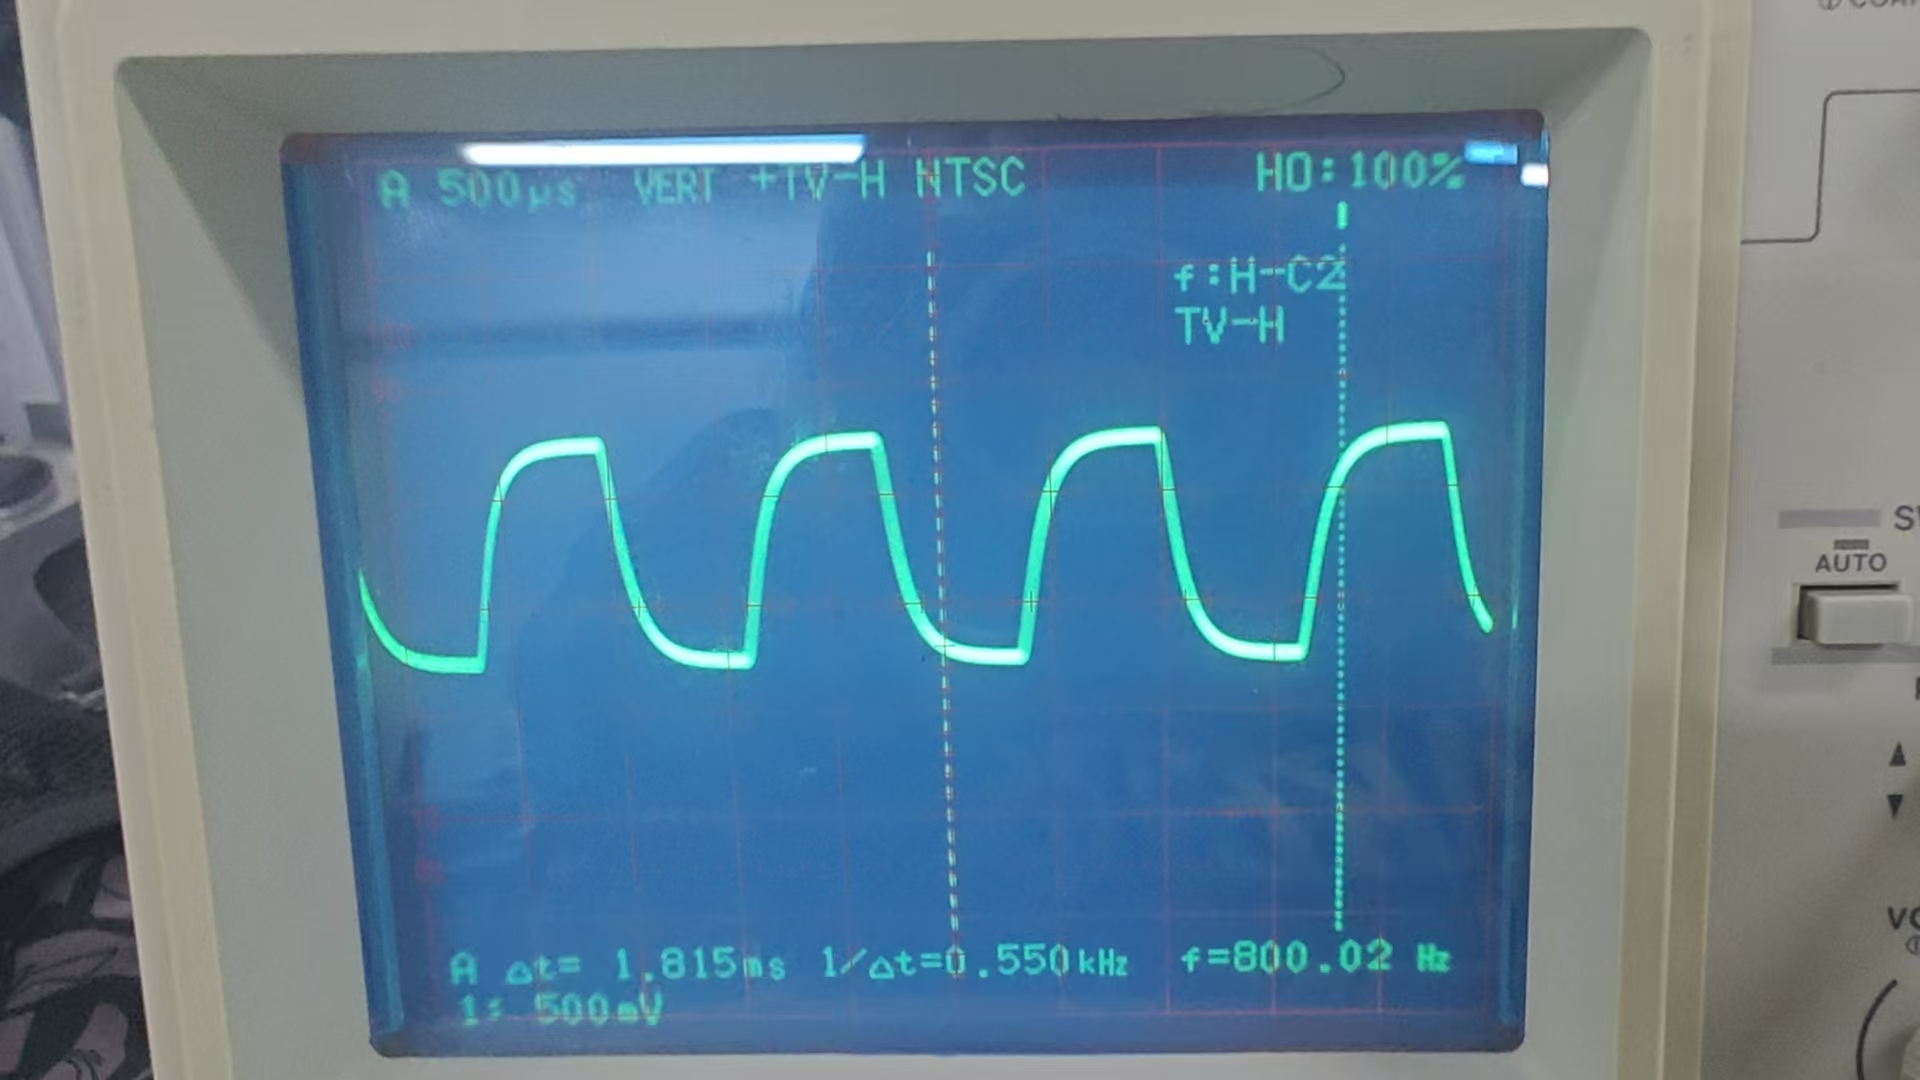
\includegraphics[width=0.55\linewidth]{RLC1000}
		\caption{$RLC1000\Omega$}
		\label{fig:rlc1000}
	\end{figure}
	\begin{figure}[H]
		\centering
		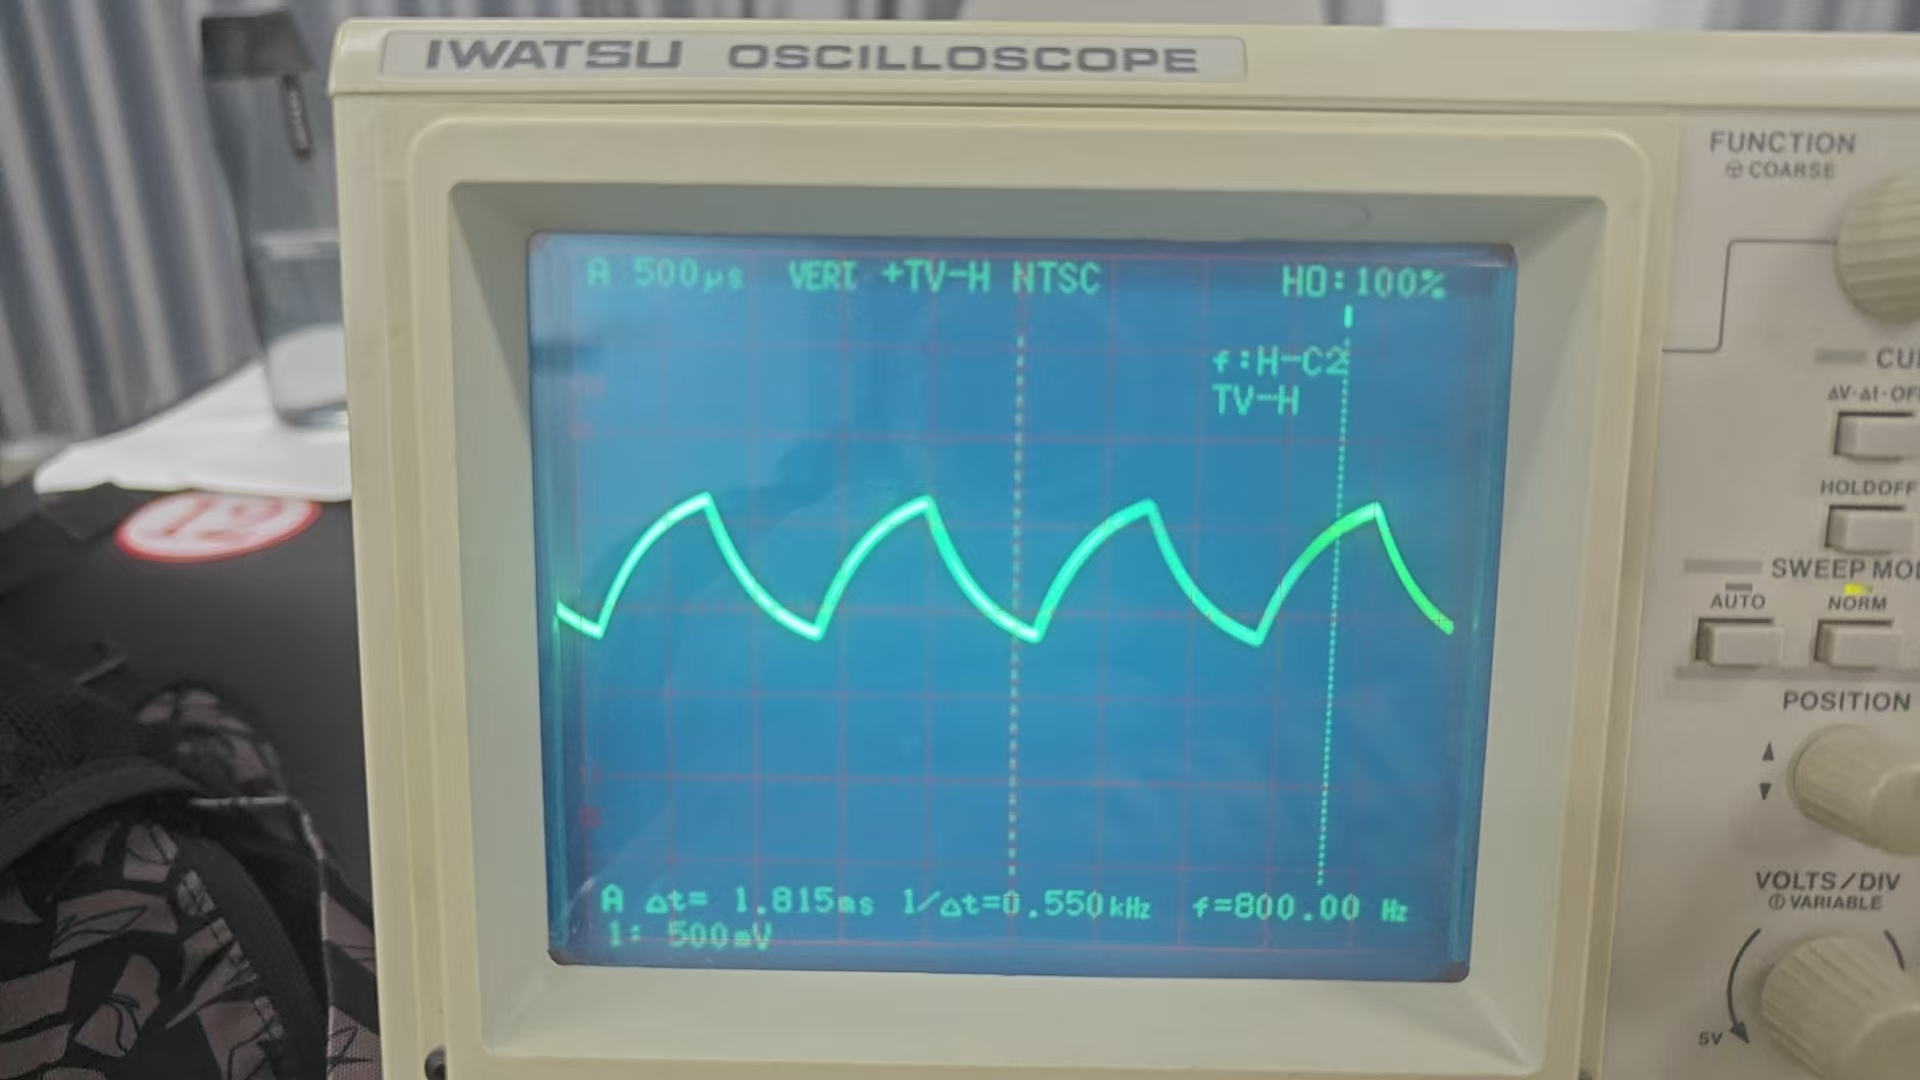
\includegraphics[width=0.55\linewidth]{RLC3000}
		\caption{$RLC3000\Omega$}
		\label{fig:rlc3000}
	\end{figure}
	我们实验的参数为$C=0.1\mu F,L=20mH$.\\
	\[4\frac{L}{C}=\frac{4\times20\times10^{-3}H}{1\times10^{-7}F}=8\times10^5\Omega^2\]
	当电阻$R=510\Omega\text{和}R=100\Omega$时,电路大致处于欠阻尼状态;当$R=1000\Omega\text{和}R=3000\Omega$时,电路处于过阻尼状态.\\
	
	以$894.427\Omega$作为标准,将波形划分为欠阻尼,临界阻尼和过阻尼状态.\\

	
	\section{数据拟合}
	\begin{figure}[H]
		\centering
		
\includegraphics[width=0.7\linewidth]{1}
		\caption{数据拟合}
		\label{fig:1}
	\end{figure}
	在充电过程中,我们可以读出$T_{0.5}=0.09ms(U_C=0.632U)$,在放电过程中,我们可以读出$T_{0.5} = 0.0955ms(U_C=0.368U)$,然后我们利用这两个数据重新画图.
	\begin{figure}[H]
		\centering
		
\includegraphics[width=0.7\linewidth]{2}
		\caption{重新绘制}
		\label{fig:2}
	\end{figure}
	理论计算:
	\[T_{0.5}=\tau ln2=RCln2=1000\Omega\times1\times10^{-7}F=0.1ms\]
	\section{指数拟合}
	我们也可以通过指数拟合得到结果.
	\subsection{充电过程}
	\begin{figure}[H]
		\centering
		
\includegraphics[width=0.7\linewidth]{4}
		\caption{充电过程}
		\label{fig:4}
	\end{figure}
	得到\[T_{0.5}=\frac{1}{11.13}ms=0.089847ms\]
	\[\text{相对误差}:\frac{0.1-0.089847}{0.1}\times100\%=10.153\%\]
	\subsection{放电过程}
	\begin{figure}[H]
		\centering
		
\includegraphics[width=0.7\linewidth]{5}
		\caption{放电过程}
		\label{fig:5}
	\end{figure}
	得到\[T_{0.5}=\frac{1}{10.84}ms=0.0922509ms\]

	\[\text{相对误差}:\frac{0.1-0.0922509}{0.1}\times100\%=7.7491\%\]

	\end{document}